\section{Preservation Planning}
As already mentioned, the preservation planning process is a well-defined workflow consisting of three phases with several steps amounting to 11 altogether \cite{STR07_jcdl}. The process specification was created during the PLANETS project and has been verfied by numerous case studies since then. 

In the first phase, \textit{``Define Requirements''}, the scope of the preservation plan is demarcated. The preservation expert has to follow three steps; to provide information about the collection, environment etc. (\textbf{Define Basis}), to choose representative sample records for experimentation (\textbf{Define Sample Records}) and to identify the requirements for the preservation plan or the so called objective tree, which summarized high-level goals of the plan (\textbf{Identify Requirements}). 

In the second phase, \textit{``Evaluate Alternatives''}, another 5 steps have to be followed. Starting with the definition of alternatives (\textbf{Define Alternatives}), the responsible preservation expert has to choose a set of potential actions, with all related informations, such as environment, tool invocation parameters, etc. In the following (\textbf{GO/NO-GO}) step a decisions is made whether to proceed or not based on each preservation action, the estimated resources and the defined requirements. After that the planner has to create suitable experiments (\textbf{Develop Experiment}), which are well-documented, repeatable set of actions with their environment and the capability to capture their results. In the following (\textbf{Run Experiment}) step, each preservation action is executed against the chosen sample records in order to obtain different results. In the last step of this phase (\textbf{Evaluate Results}) the results of the experiment output is evaluated against the objective tree in order to check if the identified requirements were met or not.

The third phase, \textit{``Consider Results''}, is responsible for the objective analysis of the results. In its first step (\textbf{Transformed Measured Value}) all experiment results are transformed into the same scale (0-5) making use of special transformation tables and utility function. The following (\textbf{Set Importance Factor}) step provides the ability to equal the weight of different parts of the requirement objective tree as not all goals are equally important. In the last step (\textbf{Analyse Results}) all measures are aggregated per objective and provide the necessary basis for a decision.

\begin{figure}[htb]
\begin{center}
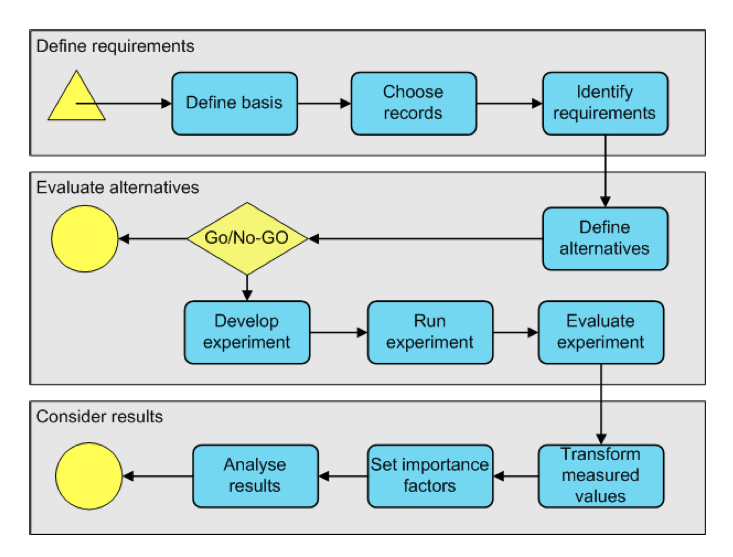
\includegraphics[width=4.5in]{figures/contentprofiling/planningworkflow.png}
\caption{Overview of PLANETS Preservation Planning workflow \cite{STR07_jcdl}.}
\label{fig:planningworkflow}
\end{center}
\end{figure}

The workflow is depicted in figure \ref{fig:planningworkflow} and provides the current state of the art in preservation planning matters. Although it provides a very solid theoretical ground and a complete specification that is working in practice, there is one flaw in the concept, which leaves space for huge errors caused by human inconpetence, lack of knowledge and understanding of the collection or even sloppiness.

As one can see from the workflow all the results strongly depend on the defined goals and the analysis of the experiments output. We assume that a preservation expert will understand the objectives of his organization. Since the identification of requirementes and the setting of the goals and objectives are very important steps that are also strongly dependent on the organizational background of the preservation expert we also assume that it is unlikely they will cause errors and misunderstandings in later steps. Also if the planner happens to choose wrong preservation action alternatives, the result will be in the worst case scenario a 'Do Nothing' alternative, which will not solve the problem at hand, but will also not do any damages.
However, there is one step that could have serious implications and even cause damages or resource loss if taken lightly. Consider the following example, where the chosen sample records are picked up at random from a medium sized collection with several thousands of objects. Then the experiments show a particular preservation action is very feasible and the planner chooses to execute this action over the whole content, due to the experiments output and the consequent analysis. Although the analysis, and the decision are perfectly valid (in their implementation and execution), it could turn out that the result of the preservation operation does not meet the requirements defined. This could happen, due to many different aspects in the format and content profile of the collection at hand. To summarize, the defined requirements and objectives are ok, the experiments are valid, the analysis is correct, but the overall results are not feasible due to the false premisse, that the random chosen set of sample records is representative.

One can argue, that no real preservation expert will choose representatives at random. Although, this might be true, there are numerous other factors that have to be considered when choosing the representatives and since the collections that are worth preserving are often big enough, the overhead for the preservation expert is just not feasible to select them by hand. Thus the representatives are usually chosen by format and format version in combination with their size (min, max and average).

The planning tool Plato, developed at the University of Technology in Vienna, implements this process and appends a fourth phase, where the user/planning expert can create an executable plan, which can be deployed within a repository. The preservation action plan is a well defined specification that serves the purpose of documentation of the decisiion and contains the executable part, which specifies the tools, environment and parameters to use during the preservation operation.

However, in its current release the planning tool supports only manual sample records definition and although it assists the planner with integrated characterization tools, it cannot provide higher certainty in the validity of the chosen representatives. It seems that integration with another tool that provides a complete content profile (generated in an automatic fashion) could provide a huge benefit to preservation planners.

\section{Collection \& Content Profiling}
% goals
% what is it c3
% jhove (identify, characterize, validate)
% why is it important (iteration of before)
% specification (representation, xml, rdf)
%...

\section{Representative Sets}
% what is the problem,
% how do we create them/find them
% ...

\section{Continuos Profiling}